% !TeX program = xelatex
\documentclass[12pt,a4paper]{article}
\usepackage{fontspec}
\setmainfont{Times New Roman}
\usepackage[english,russian]{babel}
\usepackage{amsmath,amssymb,mathrsfs,cancel}
\usepackage[margin=22mm]{geometry}
\usepackage{graphicx,float}
\usepackage[unicode,hidelinks]{hyperref}
\DeclareMathOperator{\grad}{grad}
\DeclareMathOperator{\Div}{div}
\newcommand{\Rey}{\mathrm{Re}}
\setlength{\emergencystretch}{3em}
\interfootnotelinepenalty=10000
\newcommand{\topic}[1]{\par\medskip\noindent\textbf{#1}\par\nobreak\smallskip}
\renewcommand{\thefootnote}{\arabic{footnote})}
\begin{document}
\section*{Вопрос 7}
\noindent Изотермическая фильтрация газа в недеформируемой пористой среде. Уравнение для давления (уравнение Лейбензона). Аналогия с пологими безнапорными движениями несжимаемой жидкости в пористой среде.

\medskip
\noindent\textbf{Источник:} Н. Е. Леонтьев. \textit{Основы теории фильтрации}. 2-е изд. Москва: МАКС Пресс, 2017. Глава III, § 11, печатные страницы 66--69.
\par\bigskip
% Источник: Leontiev-2017.pdf; печатная страница: 66; страница файла: 66
\section*{Глава III. Фильтрационные течения с учетом сжимаемости флюида и пористой среды}
\subsection*{§ 11. Изотермическая фильтрация газа в недеформируемой пористой среде}
\topic{Уравнение Лейбензона}
\setcounter{footnote}{0}
При фильтрации газа в промысловых условиях становятся существенными эффекты, связанные с сжимаемостью флюида. В первом приближении можно пренебречь сжимаемостью пористого скелета по сравнению с сжимаемостью газа\footnote{Обычно упругие модули материала скелета (например, модуль Юнга $E$) на много порядков больше давления газа, поэтому относительное изменение удельного объема газа $\delta V/V\sim\delta p/p$ много больше относительных деформаций материала скелета $\varepsilon_{ij}\sim\delta p/E$, вызванных изменениями давления газа.}, считая пористость и проницаемость известными функциями только от пространственных координат:
\[m=m(x,y,z),\qquad k=k(x,y,z),\]
а движение газа (в отсутствие дополнительных источников тепловой энергии) считать \textit{изотермическим}:
\[T(x,y,z,t)=T_0=\mathrm{const}.\]
В этом случае замкнутая система уравнений состоит из уравнения неразрывности и закона Дарси\footnote{Действием массовых сил при фильтрации газа можно пренебречь.}
\[m\frac{\partial\rho}{\partial t}+\Div(\rho\boldsymbol{u})=0,\qquad\boldsymbol{u}=-\frac{k}{\mu}\grad p,\]
к которым добавляются известные уравнения состояния для газа:
\[\rho=\rho(p,T_0)=\rho(p),\qquad\mu=\mu(p,T_0)=\mu(p).\]
Из этих уравнений можно получить одно уравнение относительно давления. Действительно, подставляя закон Дарси в уравнение неразрывности и для простоты полагая пористость и проницаемость постоянными величинами, получим уравнение
\[m\frac{d\rho(p)}{dp}\frac{\partial p}{\partial t}=k\Div\left(\frac{\rho(p)}{\mu(p)}\grad p\right),\]
% Источник: Leontiev-2017.pdf; печатная страница: 67; страница файла: 67
которое после введения \textit{функции Лейбензона}\setcounter{footnote}{0}\footnote{Функция Лейбензона монотонно возрастает, и, следовательно, может быть обращена: $p=p(\mathscr{P})$.}
\[\mathscr{P}(p)=k\int_0^p\frac{\rho(p_1)}{\mu(p_1)}\,dp_1\]
приобретает вид нелинейного уравнения относительно $\mathscr{P}$:
\[\frac{\partial\mathscr{P}}{\partial t}=\varkappa(\mathscr{P})\cdot\triangle\mathscr{P},\quad\varkappa(\mathscr{P})=\varkappa(\mathscr{P}(p))=\frac{k\rho(p)}{m\mu(p)}\frac{dp(\rho)}{d\rho}.\]
Обратим внимание, что функции $\mathscr{P}(p)$ и $\varkappa(p)$ зависят только от свойств газа и являются \textit{известными} до решения задачи.

В частном случае газа с уравнением состояния Менделеева--Клапейрона и постоянной вязкостью $\mu=\mathrm{const}$\footnote{Вязкость газа из невзаимодействующих частиц, как это устанавливается в молекулярно-кинетической теории, не зависит от давления и увеличивается с ростом температуры по закону $\mu\sim\sqrt T$. Вязкость реальных газов при $T=\mathrm{const}$ как правило возрастает с повышением давления.} эти формулы дают
\[\begin{gathered}
p=\frac{p_0}{\rho_0}\rho,\quad\mathscr{P}(p)=\frac{k\rho_0}{2\mu p_0}p^2,\quad\varkappa(\mathscr{P}(p))=\frac{k}{m\mu}p,\\
\frac{\partial(p^2)}{\partial t}=\frac{k}{m\mu}p\triangle(p^2),
\end{gathered}\]
откуда получается \textit{уравнение Лейбензона}\footnote{Уравнение (11.1) было получено в начале 1920-х гг. академиком Л.С.Лейбензоном и несколько позже американским гидромехаником М.Маскетом (M.Muskat).}
\begin{equation}\frac{\partial p}{\partial t}=\frac{k}{2m\mu}\triangle(p^2),\tag{11.1}\label{q7:eq-11-1}\end{equation}
которое совпадает с уравнением Буссинеска (9.3) для формы пологой поверхности депрессии при безнапорной фильтрации несжимаемой жидкости.
\topic{Граничные условия}
При постановке краевых условий для уравнения Лейбензона нужно переформулировать обсуждавшиеся в § 6 соотношения в терминах давления. На \textit{непроницаемой границе} в силу закона Дарси выполняется
% Источник: Leontiev-2017.pdf; печатная страница: 68; страница файла: 68
условие $\frac{\partial p}{\partial n}=0$, на \textit{границе со свободным газом} (например, при выходе в атмосферу газа из пласта) ставится условие постоянства давления $p=\mathrm{const}$. При \textit{выходе газа в ствол скважины}, которая моделируется отрезком прямой, могут задаваться интегральные характеристики, например объемный расход газа, выражаемый поверхностным интегралом от $\frac{\partial p}{\partial n}$.
\setcounter{figure}{24}
\begin{figure}[H]\centering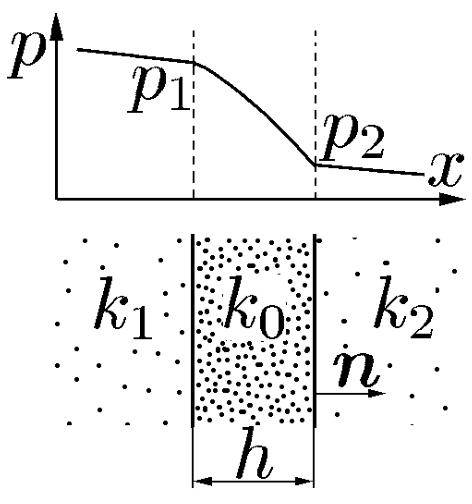
\includegraphics[width=.26\linewidth]{figures/figure-25.png}\caption{}\label{q7:fig-25}\end{figure}
Еще одним примером границы является \textit{тонкая низкопроницаемая прослойка} между двумя высокопроницаемыми пластами. Общее условие постоянства массового расхода $[\rho(p)k/\mu(p)\cdot\frac{\partial p}{\partial n}]=0$ в силу непрерывности давления на разрыве приводит к соотношению $[k\frac{\partial p}{\partial n}]=0$. Если проницаемость промежуточного пласта $k_0$ много меньше проницаемостей $k_1$ и $k_2$ соседних пластов, то прослойка будет играть роль сопротивления, при фильтрации через которое образуется большой перепад давления (рис.~\ref{q7:fig-25}). Пользуясь малой толщиной $h$ прослойки, можно приближенно использовать внутри нее распределение давления при стационарном одномерном течении газа, что дает два условия
\[\left.k_1p_1\frac{\partial p}{\partial n}\right|_1=k_0\frac{p_2^2-p_1^2}{2h}=\left.k_2p_2\frac{\partial p}{\partial n}\right|_2,\]
где индексами «1» и «2» обозначены (неизвестные) параметры газа с обеих сторон от прослойки\setcounter{footnote}{0}\footnote{В первом издании этого учебного пособия граничные условия были приведены с ошибкой, которую нам любезно указал С. А. Пославский.}.
\topic{Автомодельная задача о закачке газа в пласт}
В качестве примера использования уравнения Лейбензона рассмотрим одномерную задачу о закачке газа в полубесконечный пласт (Г.И.Баренблатт, 1952). Предположим, что в начальный момент давление газа в пласте пренебрежимо мало: $p(x,0)=0$, а во входном сечении пласта $x=0$ давление поднимается по линейному закону: $p(0,t)=\alpha t$, $\alpha=\mathrm{const}$ (рис.~\ref{q7:fig-26}~\textit{а}). После начала закачки по пласту будет распространяться волна повышения давления, описываемая уравнением
\begin{equation}p'_t=K(p^2)''_{xx},\qquad K=\frac{k}{2m\mu}=\mathrm{const},\tag{11.2}\label{q7:eq-11-2}\end{equation}
% Источник: Leontiev-2017.pdf; печатная страница: 69; страница файла: 69
причем на бесконечности возмущение давления должно стремиться к нулю: $p(x,t)\to0$ при $x\to\infty$.

Общий вид зависимости давления от времени и координаты устанавливается с помощью $\pi$-теоремы и имеет вид
\[p=p(x,t,K,\alpha)=\alpha t\cdot f(\xi),\qquad\xi=\frac{x}{t\sqrt{K\alpha}},\]
после чего нахождение решения \eqref{q7:eq-11-2} с учетом начальных и граничных условий сводится к краевой задаче
\[f(\xi)-\xi f'(\xi)=(f^2(\xi))''_{\xi\xi},\quad f(0)=1,\quad f(\infty)=0.\]
\begin{figure}[H]\centering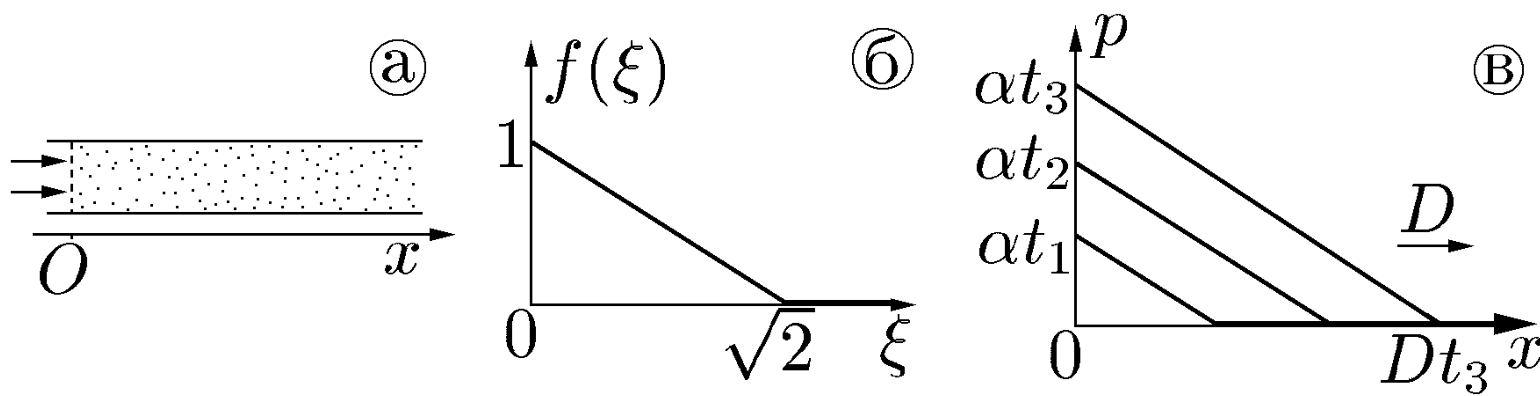
\includegraphics[width=.85\linewidth]{figures/figure-26.png}\caption{}\label{q7:fig-26}\end{figure}
Можно заметить, что дифференциальное уравнение относительно $f(\xi)$ имеет решение вида $f(\xi)=A+B\xi$, где $A=2B^2$, причем из граничного условия при $\xi=0$, соответствующего входу в пласт, получается $A=1$, $B=\pm1/\sqrt2$. Решение, соответствующее знаку плюс, стремится к бесконечности и не удовлетворяет второму граничному условию при $\xi\to\infty$, а решение, отвечающее знаку минус, обращается в ноль при $\xi=\sqrt2$ и может быть продолжено за эту точку тождественным нулем (рис. 26~\textit{б}). При этом будут выполнены условие на бесконечности и, как в этом можно убедиться, соотношения (6.3) (с нулевыми источниковыми членами в правых частях) на слабом разрыве, соответствующем $\xi=\sqrt2$.

Таким образом, решение задачи имеет вид
\[p(x,t)=\begin{cases}\alpha t-\sqrt{\alpha/(2K)}x&\text{при }x\leqslant t\sqrt{2K\alpha},\\0&\text{при }x>t\sqrt{2K\alpha},\end{cases}\]
причем передний фронт возмущения распространяется с \textit{конечной} скоростью $D=\sqrt{2K\alpha}=\sqrt{\alpha k/(m\mu)}$. Качественный вид зависимости $p(x)$ для трех моментов времени $t_1<t_2<t_3$ показан на рис. 26~\textit{в}.
% Конец § 11. На странице 70 начинается § 12.

\end{document}
